\onehalfspacing
\section{Implementierung}
In diesem Kapitel werden die verschiedenen Implementierungsschritte erläutert. Beispielhaft wird auf einzelne Schlüsselstellen eingegangen und die entsprechenden Lösungsstrategien hierfür beschrieben. Weiterhin wird kurz  erläutert welche Programmierumgebung bzw. Sprache verwendet wurde. Da es sich bei der Implementierung um ein Proof of Concept handelt, werden nicht alle Softwarekomponenten aus dem erstellten Konzept implementiert. Bei der Implementierung dienen die Regeln des Clean Code Development als Grundlage \cite{CleanCodeDevelopment.2015}. Auch wird bei der Implementierung auf die Einhaltung der Programming Principles wie DRY, KISS, SOLID etc. geachtet. Als Code Management System wird ein GitLab Repository verwendet. Dies bietet Schutz gegen Dateiverlust und ermöglicht eine Versionierung der Software. Für das verfassen von Kommentaren werden die Doxygen Richtlinien angewendet. Dies ermöglicht später die automatische Generierung einer entsprechenden Code Dokumentation.
	\subsection{Entwicklungsumgebung/Programmiersprache}
	Die Auswahl der Programmiersprache gestaltete sich aufgrund der Anforderung zur Integrationsfähigkeit in das Automated Testing @ GBC07  Projekt relativ einfach. Durch das Projekt Automated Testing @ GBC07  wird als Programmiersprache ITE vorgegeben. Da ITE eine objektorientierte Sprache ist, ähneln die meisten Sprachkonstrukte denen von C++. Jedoch sind bestimmte Funktionalitäten wie zum Beispiel Interfaces in ITE noch nicht implementiert. Als Entwicklungsumgebung kommt Visual Studio Code zum Einsatz. Hier ist die Integration des ITE Compilers sehr einfach. Weiterhin ist Visual Studio Code einfach zu bedienen und kostenlos verfügbar. 
	\newpage
	\subsection{Hiperface Implementierung}
	Die Hiperface Komponente ist im späteren Einsatz für die Kommunikation mit dem \ac{MFB} zuständig. Durch diese Aufgabe stellt sie die Kernkomponente der Testsuite dar. Da außerhalb der Hiperface Schnittstelle keine Möglichkeit zur Kommunikation, oder Datenaustausch mit dem zu testenden \ac{MFB} besteht. Durch die Kozeptionierung ist eine entsprechende Klassenstruktur für die Implementierung vorgegeben (siehe \dq \nameref{fig:Klassen_Hiperface.jpg}\dq). Bei der Umsetzung der konkreten Funktionen kann teilweise auf bestehenden Code zurückgegriffen werden. Dies bietet den Vorteil, dass zum Beispiel die einzelnen Hiperface Befehle nicht von Grund auf neu implementiert, sondern lediglich angepasst und in die neue Softwarearchitektur integriert werden müssen. Diese Befehle werden in der \dq HiperfaceBaseFunctions\dq~Klasse zusammengefasst. Die \dq HiperfaceUserFunctions\dq~Klasse enthält zusammengesetzte Funktionen, welche auf die Funktionen der \dq HiperfaceBasFunctions\dq~Klasse zugreifen. Dies geschieht mittels einer klassischen objektorientierten Programmierung und der Erzeugung eines Objekts vom Typ \dq HiperfaceBaseFunctions\dq. Ein Beispiel für dieses Vorgehen ist die Abfrage des LED Current. In Listing \dq \nameref{lst:checkCurrent}\dq~ist zu erkennen, wie der Aufruf der Funktion \dq RAnalogValue\dq~mit dem entsprechenden Übergabeparameter stattfindet. Auch ist hier zu erkennen, dass bei jedem Befehl geprüft wird, ob bereits eine Initialisierung der Schnittstelle stattgefunden hat.
\newline
\begin{center}

\begin{minipage}[h]{\textwidth}
	\lstinputlisting[language = java, style = customc, label={lst:checkCurrent}, caption = {Auslesen eines Analogwertes}]{Listings/checkCurrent.txt}
\end{minipage}

\end{center}
Die Implementierung der entsprechenden Hiperface Befehle erfolgt in der \dq HiperfaceBaseFunctions\dq~Klasse. Es wird zwischen lesenden und schreibenden Befehlen unterschieden. Der Aufbau der verschiedenen Befehle ist entsprechend der jeweiligen Kategorie sehr ähnlich. Ein Beispiel für einen lesenden Befehl ist die Abfrage des \ac{MFB} Status.
\newline
\begin{center}

\begin{minipage}[h]{\textwidth}
	\lstinputlisting[language = java, style = customc, label={lst:uutRStatus}, caption = {Abfragedes aktuellen Geräte Status}]{Listings/uutRStatus.txt}
\end{minipage}

\end{center}
Das Listing \dq \nameref{lst:uutRStatus}\dq~zeigt den entsprechenden Quellcode. Das Hiperface Kommando setzt sich aus dem Befehl (Angabe als Hex-Code) sowie der Angabe das eine Antwort erwartet wird (bool) zusammen. Im Anschluss wird die Funktion \dq Hiperface\_Execute\dq~aufgerufen und ihr das Kommando als Parameter (struct) übergeben. Die \dq Hiperface\_Execute\dq~Funktion übernimmt dann das Berechnen der Checksumme, sowie das Senden des Befehls an das \ac{MFB}. Hierbei wird das von der Klasse \dq HiperfaceComInterface\dq~zur Verfügung gestelltes Interface genutzt.\newline

Durch die objektorientierte Programmierung besteht die Möglichkeit mehrere Instanzen der Hiperface Schnittstelle zu erzeugen. Da dies für den späteren Gebrauch jedoch nicht zielführend ist und es hierdurch zu Schwierigkeiten bei der Verwendung der COM Ports kommen kann, wird das Erzeugen mehrerer Instanzen der Klasse \dq HiperfaceComInterface\dq~mittels eines Singelton Entwurfsmusters verhindert. Die Implementierung ist in Listing \dq \nameref{lst:singelton}\dq~zu sehen.	 
\newline
\begin{center}

\begin{minipage}[h]{\textwidth}
	\lstinputlisting[language = java, style = customc, label={lst:singelton}, caption = {Beispiel Singelton Entwurfsmuster}]{Listings/singelton.txt}
\end{minipage}

\end{center}
Durch das Singelton Pattern wird sichergestellt, dass eine Klasse nur genau ein Exemplar besitzt. Darüber hinaus stellt es einen globalen Zugriffspunkt auf dieses dar.\cite{Gamma.2008} Die Implementierung des Singelton erfolgt hier durch das deklarieren des Konstruktors als \dq Privat\dq. Somit ist kein Zugriff von außerhalb der Klasse auf ihn möglich. Der Zugriff auf den Konstruktor erfolgt im Anschluss über die Funktion \dq getInstance\dq. In dieser Funktion wird geprüft, ob es bereits ein Objekt der Klasse gibt. Falls nicht, wird ein neues erstellt und dieses zurückgegeben. Ein Zugriff auf die Klasseninstanz ist in Listing \dq \nameref{lst:zugriffSingelton}\dq~zu sehen.
\newline
\begin{center}

\begin{minipage}[h]{\textwidth}
	\lstinputlisting[language = java, style = customc, label={lst:zugriffSingelton}, caption = {Beispiel Zugriff Singelton }]{Listings/zugriffSingelton.txt}
\end{minipage}

\end{center}
Die Verwendung des Singelton Entwurfsmusters ist teilweise umstritten, da es zum Beispiel die Anwendung von Unit Tests erschwert, jedoch ist es komfortabel und unkompliziert zu implementieren. Weiterhin bietet es die Möglichkeit sehr gut zu Steuern und zu Kontrollieren wann auf die Instanz zugegriffen wird. 
\subsection{Motor Implementierung}
	Bei vielen Testfällen wird neben den Hiperface Befehlen auch ein Motor benötigt um die Welle des \ac{MFB} zu 		drehen und so entsprechende Messdaten zu erhalten. Die Motoren verfügen über entsprechende 						Schnittstellen, welche es dem Benutzer ermöglichen, diese mittels einer Seriellen COM Schnittstelle zu 			steuern. Bei der Implementierung der Motorfunktionalität wird besonderen Wert auf die Erweiterbarkeit 			gelegt. Im Moment sind zwei verschiedene Motoren am Teststand vorhanden. Jedoch ist eine Erweiterung dieses Bereichs in Zukunft möglich. Dieser Umstand wurde bereits bei der Kozeptionierung eingeplant und wird 			auch bei der Implementierung beachtet. Um dem Benutzer einheitliche Funktionen zur Verfügung zu stellen, 	sodass dieser im Betrieb später nicht die Motorspezifischen Befehle verwenden muss, wird hier auf überladenen Funktionen (virtuelle Funktionen) und somit polymorphe Funktionsaufrufe				gesetzt. Durch dieses Vorgehen wird das Prinzip der Protected Variations erfüllt. In der \dq EngineDriver\dq~Klasse werden die virtuellen Funktionen definiert. In Listing \dq \nameref{lst:virtFunktionen}\dq~ist ein Teil der virtuellen Funktionen, welche jeder verwendete Motoren zur Verfügung stellen muss, zu sehen.
\newline
\begin{center}

\begin{minipage}[h]{\textwidth}
	\lstinputlisting[language = java, style = customc, label={lst:virtFunktionen}, caption = {Virtuelle Methoden des Motors }]{Listings/virtFunktionen.txt}
\end{minipage}

\end{center}
In den Klassen \dq FaulhaberEngineDriver\dq~und \dq MetronixEngineDriver\dq~findet die konkrete Implementierung der entsprechenden Funktionen statt. Die beiden Klassen leiten jeweils von \dq EngineDriver\dq~ab. Ein Beispiel hierfür ist in Listing \dq \nameref{lst:impVirtFunktionen}\dq~zu sehen.
\begin{center}

\begin{minipage}[h]{\textwidth}
	\lstinputlisting[language = java, style = customc, label={lst:impVirtFunktionen}, caption = {Faulhaber Implementierung der virtuellen Funktionen }]{Listings/impVirtFunktionen.txt}
\end{minipage}
\end{center}
Um die Erzeugung der unterschiedlichen Implementierungen zu realisieren, wird hier das Factory Entwurfsmuster angewendet. Das Factory Entwurfsmuster definiert eine Klassenschnittstelle mit Methoden zum Erzeugen eines Objektes. Jedoch wird durch Unterklassen entschieden, von welcher Klasse das erzeugte Objekt sein soll.\cite{Gamma.2008}
Die Umsetzung des Factory Entwurfsmusters erfolgt in der Funktion \dq setupEngine\dq.
\begin{center}

\begin{minipage}[h]{\textwidth}
	\lstinputlisting[language = java, style = customc, label={lst:setupEngine}, caption = {Anwendung Factory Entwurfsmuster}]{Listings/setupEngine.txt}
\end{minipage}
\end{center}
In der Funktion \dq configureFaulhaberEngine\dq~bzw.\dq configureMetronixEngine\dq~wird im Anschluss der konkrete Aufruf bzw. die Erzeugung des entsprechenden Objektes durchgeführt. Dies ist in Listing \dq \nameref{lst:configFaul}\dq~zu sehen.
\begin{center}

\begin{minipage}[h]{\textwidth}
	\lstinputlisting[language = java, style = customc, label={lst:configFaul}, caption = {Erzeugung eines Faulhaber Motor Objekts}]{Listings/configFaul.txt}
\end{minipage}
\end{center}
\newpage
Durch die Verwendung des Factory Entwurfsmusters ergibt sich eine Architektur wie in Abbildung \dq \nameref{fig:ArchitekturFactory.jpg}\dq. Am linken Rand sind die entsprechenden Schichten der Architektur abgebildet. Die den Schichten zugeordneten Module, sowie deren Relationen sind daneben zu sehen. Aus Gründen der Lesbarkeit wird auf die Auflistung der Klassenmethoden und Variablen verzichtet.
\begin{figure}[h]
	\centering
  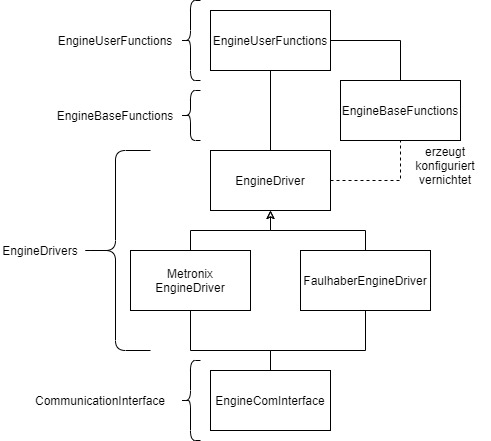
\includegraphics[width=1\textwidth]{img/ArchitekturFactory.jpg} 
   \caption{Architektur durch Factory Entwurfsmuster}
  \label{fig:ArchitekturFactory.jpg}
\end{figure}

 